\lab{Applications}{Data Visualization}{Data Visualization} 
\objective{Use data visualizations to explore data and communicate it to others.}
\label{lab:DataVis}

\section*{What is data visualization?} 
Data visualizations (or graphs) are used to understand and explore data as well as communicate results to others. 
Just as a picture is worth a thousand words, a graph is much easier than a thousand data points for the human mind to interpret. 
Though anyone working with data benefits from graphing it, data visualization is also an independent field that studies the interplay between mathematics, statistics, and the visual arts.

\section*{Types of visualizations}
There are many standard ways to visualize data, and some consistently reveal and communicate the most information about certain kinds of data sets. 
Here are some standard plots and some examples of data they are commonly used to visualize.

\begin{enumerate}
\item A \emph{scatter plot} graphs $(x,y)$ tuples as points. 
A scatter plot can reveal correlation (or lack thereof) between $x$ and $y$. 
Use a scatter plot when your data is not ordered. 
You can create a scatter plot in matplotlib with the command \li{plt.scatter()}.

\item A \emph{line plot} graphs $(x,y)$ tuples as points and then connects them with a line. 
You should use a line plot when there is a natural order to your tuples. 
For example, use a line plot to look for trends over time. 
Recall that you can create a line plot in matplotlib with the command \li{plt.plot()}.

\item A \emph{histogram} (or bar graph) depicts $(x,y)$ tuples as rectangles whose length is determined by $y$ (see Figure \ref{fig:healthcare}). 
Like line plots, histograms can be used to look for trends over time. 
Another use of a histograms is to investigate statistical distributions. 
You can create a histogram in matplotlib with the command \li{plt.hist()}. 
%TODO: Add a problem that requires them to build a histogram

\item A \emph{pie chart} depicts parts of a whole as slices of a circle. 
Often, a pie chart is best replaced with a histogram. 
This is because it is difficult for us to see how similar slices of a pie chart differ in size. 
By contrast, we can easily detect even small differences in the lengths of rectangles in a bar chart. 
However, pie charts are ideal for some purposes, especially when the exact numbers from the data are not important. 
See \cite{piecharts} for some situations where data is best represented by a pie chart. 
You can create a pie chart in matplotlib with the command \li{plt.pie()}.

\item A \emph{sparkline} is a word-sized graphic that is often embedded inline with the text. 
Created by Edward Tufte, an innovator and recognized leader in the field of data visualizations, sparklines can be used to quickly communicate large-scale trends in a data set. They are also ideal for binary data sets. 
Two sources for creating sparkplots in Python are \cite{sparkplots} and \cite{sparklineshtml}.
%TODO: Add an example of a sparkline

\item A \emph{pseudocolor plot} or heat map uses color to display a third dimension on a two-dimensional page (see Figure \ref{fig:heatmap}). 
One common use is to illustrate the temperature of an object. 
You can create a pseudocolor plot in matplotlib with the \li{plt.pcolormesh()} command.

\item \emph{Small multiples} are several minature graphics of the same type in a single visualization. 
Like sparklines, they were pioneered by Edward Tufte. Any of the plots discussed so far may be assembled into a small multiple. 
Small multiples are useful for viewing trends over time, when the data associated to each time is more complex than a single number. 
More generally, they can be used to compare many sets of similar data (\cite{tufte1990} p. 67). 
Figure \ref{fig:log_plots} could be called a small multiple, though frequently they contain more subplots. 
Recall that this kind of plot can be created in matplotlib with the command \li{plt.subplot()}.
\end{enumerate}



\section*{Exploring data with visualizations}
When you visualize data you may notice trends that are not apparent from the numbers. 
The following problem is an example of this.

\begin{problem}\label{prob:anscombe}
The data sets I-IV in Table \ref{table:anscombe} are known as Anscombe's quartet. 
Each dat set has identical statistical properties. 
In each case,
\begin{itemize}
\item The mean of $x$ is 9 and the mean of $y$ is $7.5$.
\item The variance of $x$ is 11 and the variance of $y$ is 4.127.
\item The correlation between $x$ and $y$ is .816.
\item The linear regression line is $y=3+5x$.
\end{itemize}
Plot each data set. What do you notice?

\begin{table}[H]
\begin{tabular}{l l  |  l l  |  l l  |  l l }
I & & II & & III & & IV\\
x & y & x & y & x & y & x & y \\
\hline
10.0 & 8.04 & 10.0 & 9.14 & 10.0 & 7.46 & 8.0 & 6.58 \\
8.0 & 6.95 & 8.0 & 8.14 & 8.0 & 6.77 & 8.0 & 5.76 \\
13.0 & 7.58 & 13.0 & 8.74 & 13.0 & 12.74 & 8.0 & 7.71 \\
9.0 & 8.81 & 9.0 & 8.77 & 9.0 & 7.11 & 8.0 & 8.84 \\
11.0 & 8.33 & 11.0 & 9.26 & 11.0 & 7.81 & 8.0 & 8.47 \\
14.0 & 9.96 & 14.0 & 8.10 & 14.0 & 8.84 & 8.0 & 7.04 \\
6.0 & 7.24 & 6.0 & 6.13 & 6.0 & 6.08 & 8.0 & 5.25 \\
4.0 & 4.26 & 4.0 & 3.10 & 4.0 & 5.39 & 19.0 & 12.50 \\
12.0 & 10.84 & 12.0 & 9.13 & 12.0 & 8.15 & 8.0 & 5.56 \\
7.0 & 4.82 & 7.0 & 7.26 & 7.0 & 6.42 & 8.0 & 7.91 \\
5.0 & 5.68 & 5.0 & 4.74 & 5.0 & 5.73 & 8.0 & 6.89 \\
\end{tabular}
\caption{These four sets of data are known as Anscombe's quartet.}
\label{table:anscombe}
\end{table}
\end{problem}

As Problem \ref{prob:anscombe} demonstrates, a picture can reveal a data set in ways numbers can't. 
Learning from a visualization of a data set is often a recursive process. 
You must visualize the data, make observations, and then zoom, filter, or otherwise modify your visualization to further explore the data.

One issue to consider is the range. 
By choosing to plot only a portion of your data, you may be able to focus your attention on the most relevant data. 
On the other hand, you may also miss some interesting behavior in the data you didn't graph.

Another issue to consider is scale. 
For example, suppose the number of dogs kept as pets in a certain city increases from 50,000 to 55,000 over 4 years. 
This increase can appear small or large, depending on where we start the y-axis and how long we stretch out the x-axis (see Figure \ref{fig:dog_plots}).

There are many software packages that facilitate the visual exploration of data. 
One Python library is Glue (see \cite{glue}).


\subsection*{Log plots}

One good way to analyze data is to plot it on a different scale. 
Log plots in particular can reveal important structure in a data set. 
You can create a log-log plot by taking the logarithm of both the $x$- and $y$-values. 
Analogously, you can create a log-lin plot (also called a log plot) by taking the logarithm of only the $y$-values of your data set, or a lin-log plot by taking the logarithm of only the $x$-values.

As an example, let us look at the cost of health care claims. 
Our data set is bogus but created to closely resemble real-life data. 
An initial plotting of the data produces the histogram on the left in Figure \ref{fig:healthcare}. 
From this picture, it is hard to see the nature of the data---the plot just looks like a single bar. 
We may think that all health care claims are cheap. 
However, when we take the logarithm of the claims prices, we get the histogram on the right in Figure \ref{fig:healthcare}. 
Graphed on this scale, the data has a bell-shaped distribution similar to a normal distribution. 
Moreover, we see that there are some very expensive claims being submitted, though they are few. 
\begin{figure}
\centering
\begin{subfigure}{.5\textwidth}
  \centering
  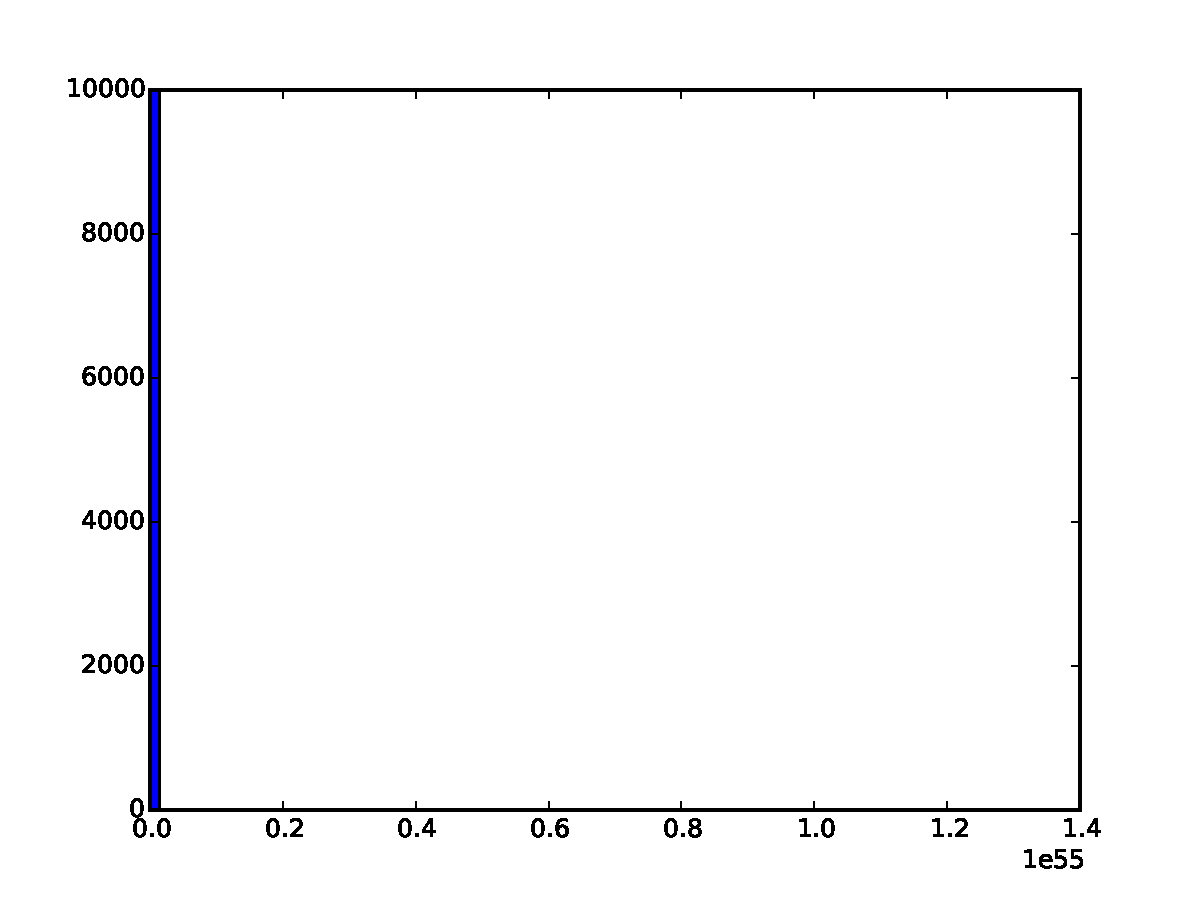
\includegraphics[width=\textwidth]{healthcare_linscale.pdf}
\end{subfigure}%
\begin{subfigure}{.5\textwidth}
  \centering
  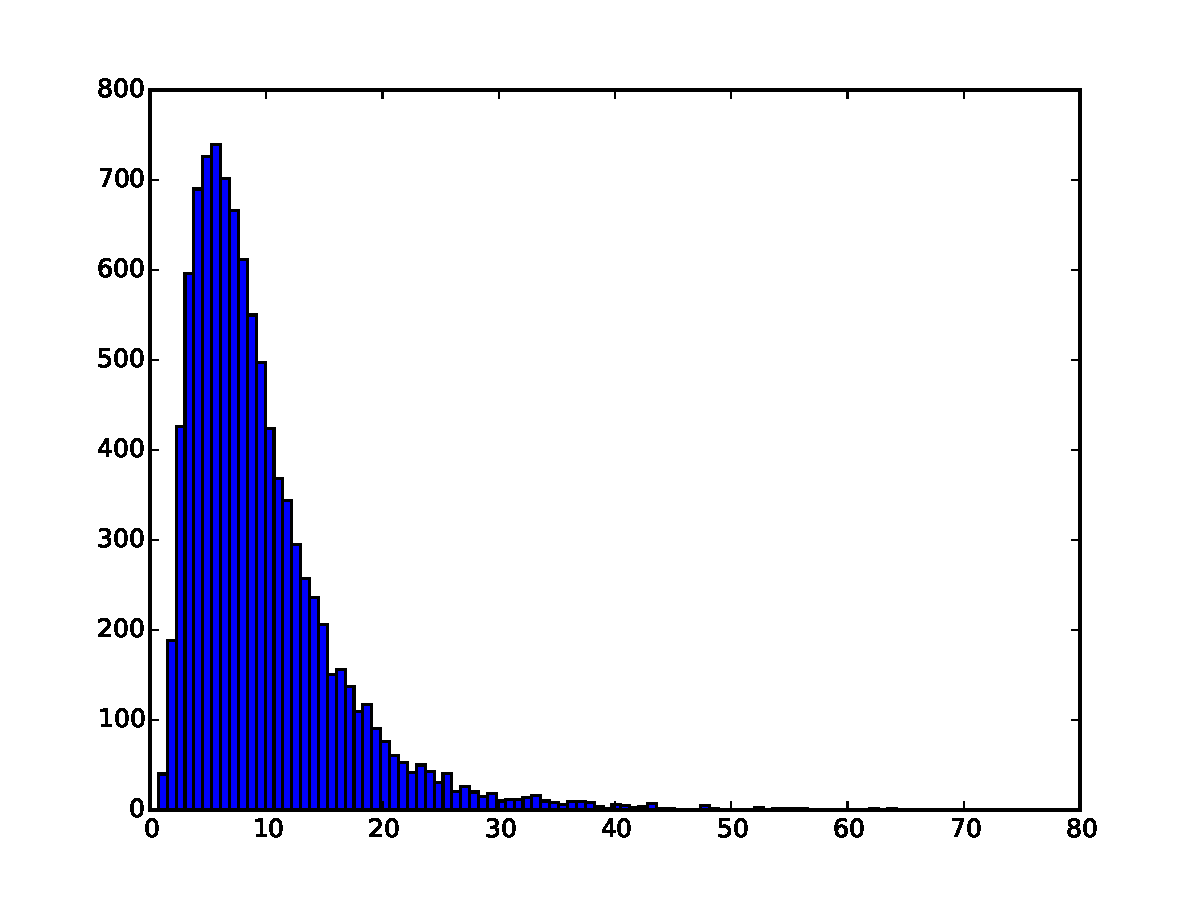
\includegraphics[width=\textwidth]{healthcare_logscale.pdf}
\end{subfigure}
\caption{The same data (meant to resemble the prices of health care claims) is plotted in both histograms above. 
The plot at left is a lin-lin scale, whereas the plot at right is a log-lin scale. 
In this case, changing scales revealed important information about the data.}
\label{fig:healthcare}
\end{figure}

As a general rule, log-lin plots are useful when the range of the $y$-values is orders of magnitude larger than the range of the $x$-values. 
Our health care data was an example of this. 
Similarly, lin-log plots are useful when the range of the $x$-values is much bigger than the range of the $y$-values. 
In any case, you can try applying a log scale to one or both of your axes as a way to explore your data.

Let us analyze the mathematics behind log plots. 
Suppose we have some data that roughly follows the line $y=cx^a$ where $c$ and $a$ are constants. 
Taking the logarithm of both sides yields
\[
\log(y) = a\log(x) + \log(c).
\]
If we set new variables $X = \log(x)$ and $Y = \log(y)$, then this equation becomes $Y = aX + \log(c)$, which is the equation of a straight line. 
So  on a log-log plot, polynomial-shaped data looks linear. 
Similarly, taking the log of $y = a^x$ yields
\[
\log(y) = \log(a)x,
\]
so exponential data looks linear on a log-lin plot. 
Finally, data of the form $y = a\log(x)+b$ will look linear on a lin-log plot. 
See Figure \ref{fig:log_plots}.

\begin{figure}
\centering
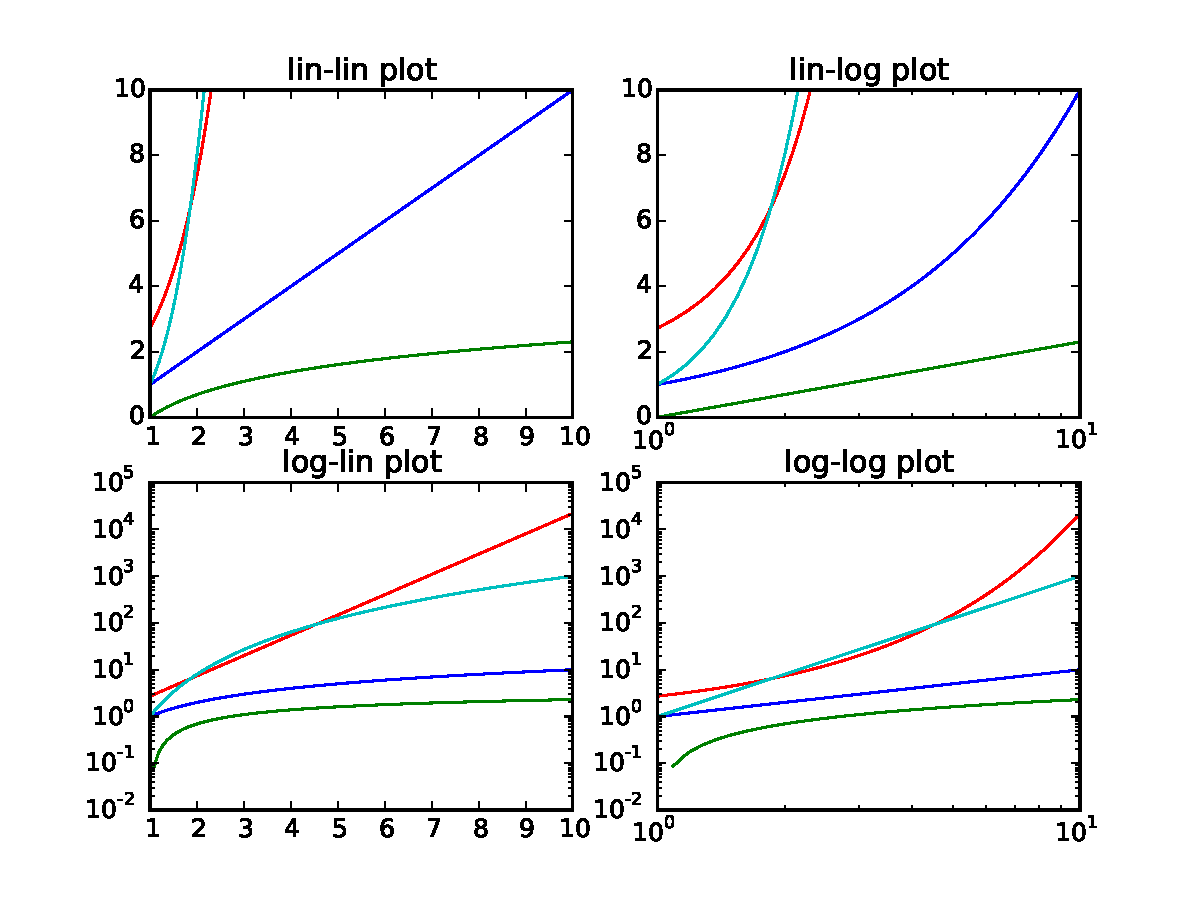
\includegraphics[width=\textwidth]{log_plots.pdf}
\caption{Here are some functions plotted on various logarithmic and linear scales. 
The dark blue line is $y=x$, the green line is $y=\log(x)$, the red line is $y=e^x$, and the light blue line is $y=x^3$. 
We have used different ranges on the $y$-axes to highlight appropriate parts of the graphs.}
\label{fig:log_plots}
\end{figure}

Be warned that many different functions can look linear on log plots. 
Thus, if you graph your data on a log-log plot and you see a line, you CANNOT conclude that your data must follow a polynomial. 
In general, you need more information.

In matplotlib, you can create plots on a logarithmic scale directly by using the \li{plt.loglog()}, \li{plt.semilogy()}, and \li{plt.semilogx()} commands. 
Their syntax is identical to that of\li{plt.plot()}. 
Alternatively, you can modify the scale of an existing plot using \li{plt.yscale()} or \li{plt.xscale()}.


\begin{problem}
Graph your data from Problem 1 in Lab \ref{lab:complexity} (Matrices and Complexity) on a (a) log-log scale, (b) log-lin scale, and (c) lin-log scale. 
In your opinion, which plot makes the data easiest to understand?
\end{problem}




\section*{Communicating data with visualizations}

As the saying has it, ``a picture is worth a thousand words.'' 
Certainly, a data visualization is far more valuable than a thousand data points to a colleague who wants to understand the results of your analysis. 
Data visualizations are critical for communication in both business and research.

\subsection*{Choosing the right visualization}
At this point, you have already used visualization to explore your data and draw conclusions, and you are ready to tell your results to someone else. 
The first step in creating a graphic to do this is to choose the right type of visualization. 
As we saw in the section ``Types of Visualizations,'' there are many possibilities, each with different strengths. 
You should carefully consider which one best suits your data set and communication needs.

\subsection*{Simplify}
Once you have chosen the visualization best suited to your data, you should design the details so that all elements contribute to the communication of data. 
Edward Tufte offers two principles for simplifying graphics: (1) erase ink that does not communicate data, and (2) erase ink that communicates data redundantly. 
Both of these principles should be applied within reason (\cite{tufte2001} pp.96-100). 

According to these principles, decorative backgrounds, fancy lettering, and cute graphics in the corner of you plots should all be deleted.

Other opportunities for simplification are harder to notice and implement. As an example, let us examine the plot on the right of Figure \ref{fig:healthcare}. 
This plot was created with the following code.

\begin{lstlisting}
import numpy as np
import scipy as sp
from matplotlib import pyplot as plt

m = 2.07
s = 0.63
num_samples = 10000
samples = []

for i in xrange(num_samples):
    samples.append(sp.random.lognormal(m, s)) 

sp_samples = sp.array(samples)

# Plot the histogram
plt.hist(sp_samples, 100)
\end{lstlisting}

For purposes of this example, the only important part of the above code is the line \li{plt.hist(sp_samples, 100)} that plots the histogram. 
What ink in this plot can we erase because it communicates no data?

First, let's get rid of the vertical black lines that separate the bars of the histograph. 
These are meaningless for our application. 
We can do this by modifying our call to \li{plt.hist()} as follows.

\begin{lstlisting}
plt.hist(sp_samples, 100, histtype="stepfilled")
\end{lstlisting}

Next, let us turn off the top and right lines that box in the graph. 
To do this, we need to access the ``axis'' object associated with the figure. 
We can access the ``axis'' object with the command \li{plt.gca()} (get current axis).

\begin{lstlisting}
# Get current axis instance
axis = plt.gca()

# Hide top and right spines
axis.spines['right'].set_visible(False)
axis.spines['top'].set_visible(False)
\end{lstlisting}

These commands only turn off the sides of the box, not the tick marks. 
To turn off the tick marks we run the following commands. 

\begin{lstlisting}
# Only show bottom and left tick marks
axis.yaxis.set_ticks_position('left')
axis.xaxis.set_ticks_position('bottom')
\end{lstlisting}

Finally, we do not need so many tick marks on the $x$- and $y$-axes. 
We adjust those along with specifying the range on each axis.

\begin{lstlisting}
# Fix x and y ranges
plt.xlim(0,70)
plt.ylim(0, 800)

# Use fewer axis ticks
plt.xticks(np.arange(0, 71, 35))
plt.yticks(np.arange(0, 801, 200))
\end{lstlisting}

The final graph is shown in Figure \ref{fig:simplify}. 
Note how much cleaner this looks than the original.

\begin{figure}
\centering
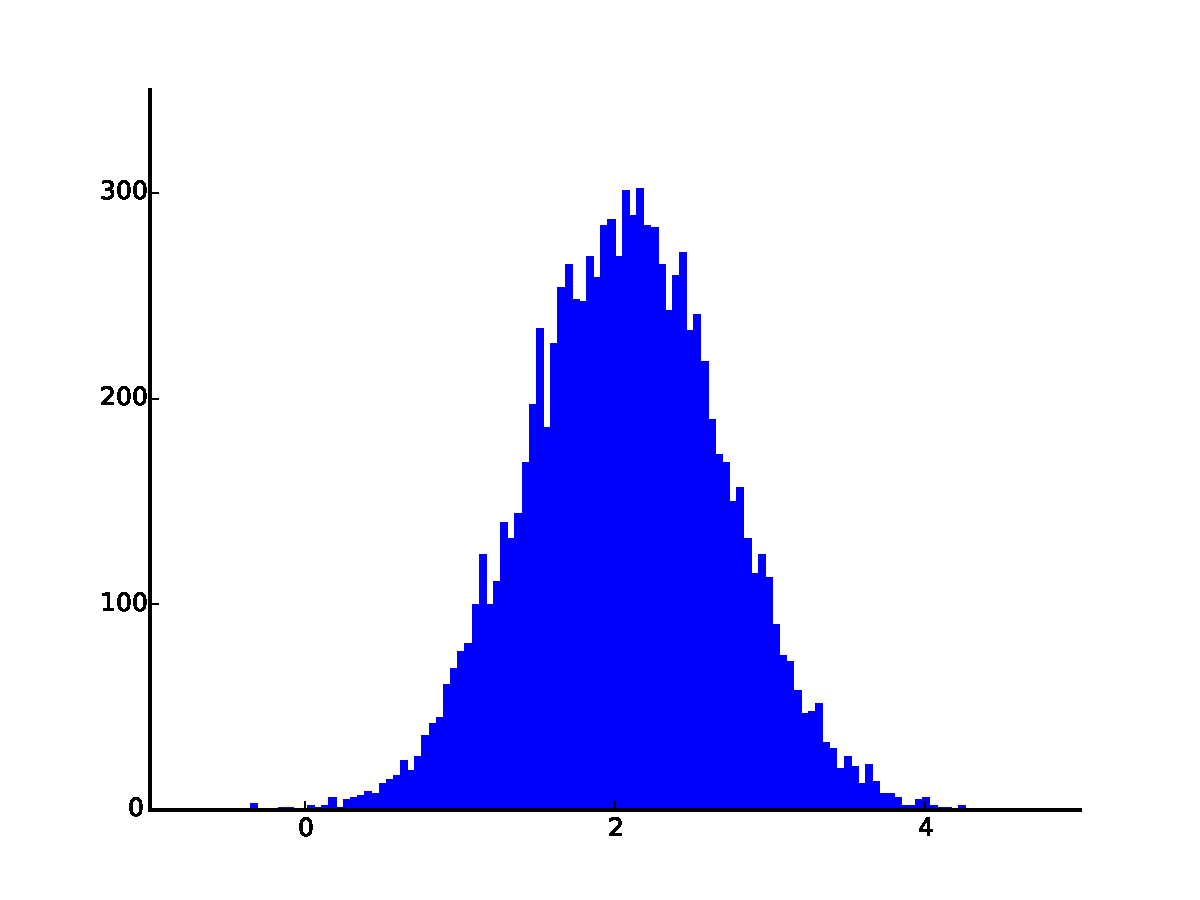
\includegraphics[width=\textwidth]{simplify.pdf}
\caption{A simplified version of the histogram in Figure \ref{fig:healthcare}.}
\label{fig:simplify}
\end{figure}


\subsection*{Color}
%TODO: explain how you can make a colorbar, either in this lab or the matplotlib lab
Color should be added to your graphic thoughtfully. 
The default settings in matplotlib should generally not be used. 
Several bright colors in a single plot often jar the viewer, so you should limit the number and intensity of colors and use them only to emphasize parts of your data. 
If a grayscale plot contains just as much information as a colored plot, consider using grayscale.

The default color settings for pseudocolor plots in matplotlib are particularly problematic. 
The default color gradient is a rainbow, which usually has no relation to the data. 
Most viewers have trouble remembering which colors are ``high" and which are ``low". 
Instead, you should set the gradient to cover one or two colors, and when possible these colors should be related to the data you are communicating. 
You can change the color gradient used by \li{plt.pcolormesh()} with the keyword argument \li{cmap} (short for ``colormap''). 
A list of predefined colormaps is available at \url{http://matplotlib.org/examples/color/colormaps_reference.html}, but you can also define your own. 
See Figure \ref{fig:heatmap} for an example of a good and bad pseudocolor plot.


\begin{figure}
\centering
\begin{subfigure}{.5\textwidth}
  \centering
  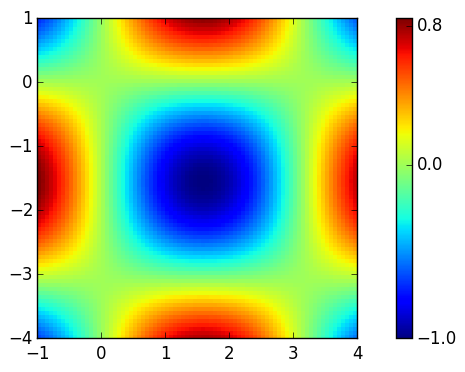
\includegraphics[width=\textwidth]{heatmap_color.png}
\end{subfigure}%
\begin{subfigure}{.5\textwidth}
  \centering
  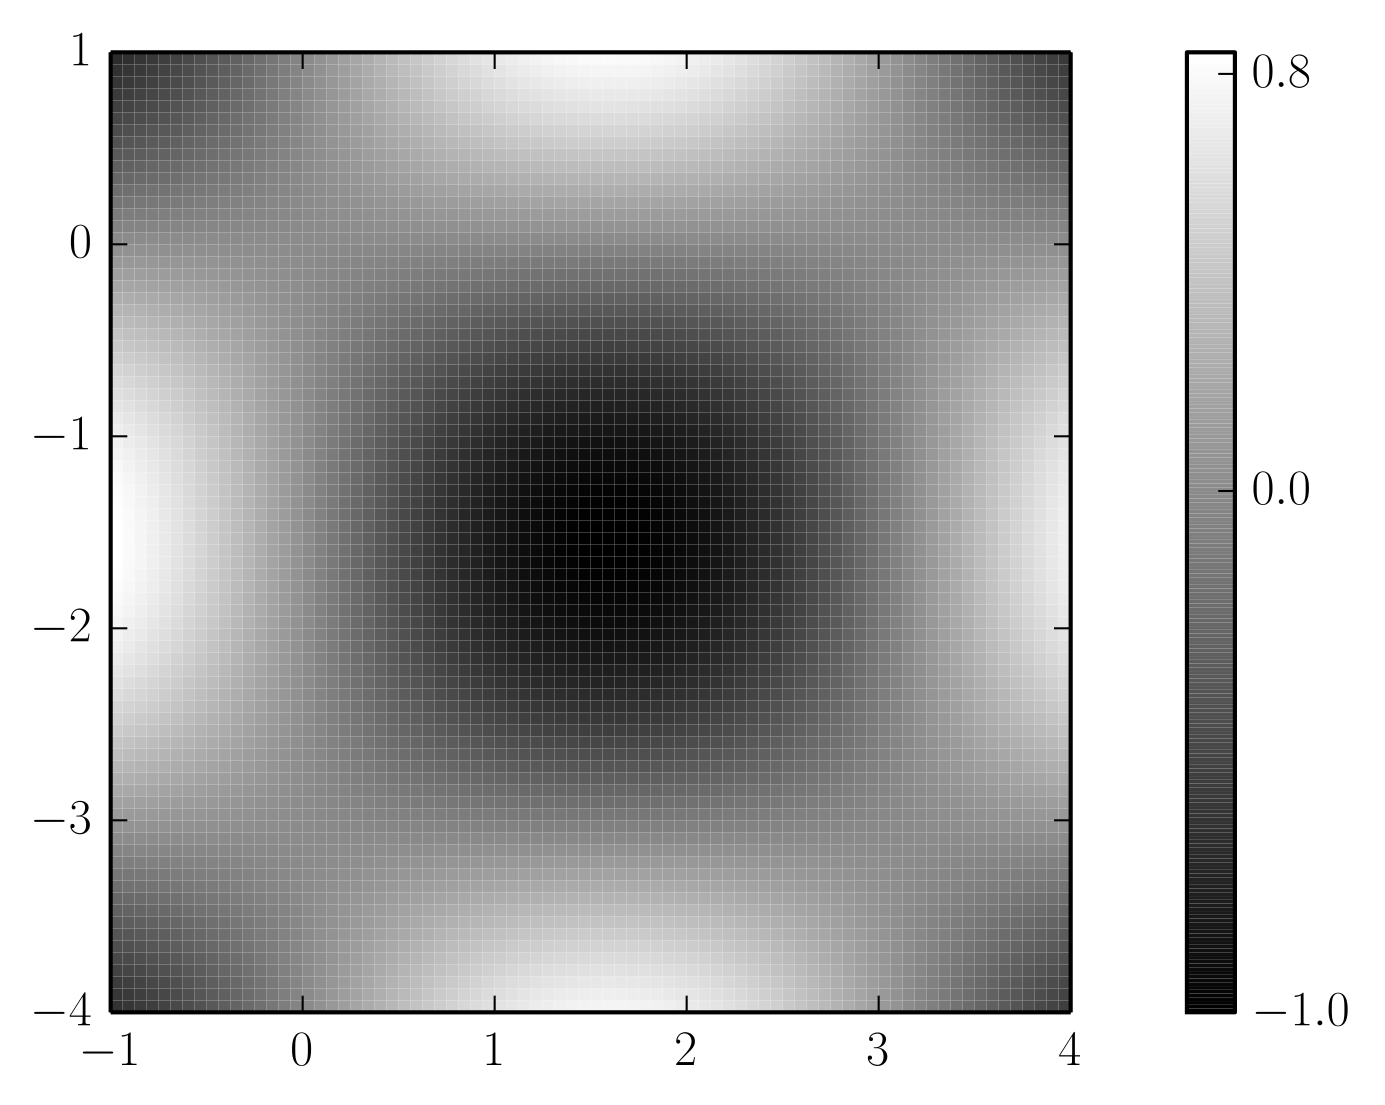
\includegraphics[width=\textwidth]{heatmap_gray.png}
\end{subfigure}
%\includegraphics[width=\textwidth]{heatmap.png}
\caption{Both of these pseudocolor plots depict the function $z = sin(x)sin(y)$ on the domain $[-1,4] \times [-4,1]$. 
The plot at left uses a rainbow gradient which has no relationship to the data. 
The plot at right uses a greyscale, which has two benefits: the colors are not irritating, and ``black'' is associated with ``low.''}
\label{fig:heatmap}
\end{figure}

%TODO: Rewrite this problem to use a specific image with a specific context
\begin{problem}
Choose a graph you previously created that you think could use simplification. 
Apply at least 3 of the following to simplify your plot:
\begin{enumerate}
\item Turn off some of the spines.
\item Fix the x or y range to better fit your data.
\item Change the number of x or y ticks.
\item Choose a better color scheme.
\end{enumerate}
Simplify your image in any other ways you can think of.
\end{problem}

\subsection*{Tell the truth}

Just as graphics can tell your reader about your data, they can also give your viewer false impressions. 
You should never use data visualization to mislead your reader. 
There are many ways pictures can be used to lie, and some of them can be unintentional.

For example, if we see differences in shapes by area, not width or height. 
Suppose you are creating a pictogram to demonstrate the recent increase in housing prices, which have doubled in the last $n$ years. 
So, you draw two houses, one that is 1'' wide and one that is 2'' wide. 
To a reader, it will appear that housing prices have increased by a factor of $2^2=4$. 
Hence, you should make pictures proportional in \emph{area} to the numbers they represent.

Scale is also important when you are drawing a line graph or a histogram. 
Differences between data points can appear small if you zoom out, or large if you zoom in (see Figure \ref{fig:dog_plots}). 
Also, changing the scale partway along the $x$- or $y$-axis can distort data.

\begin{figure}
\centering
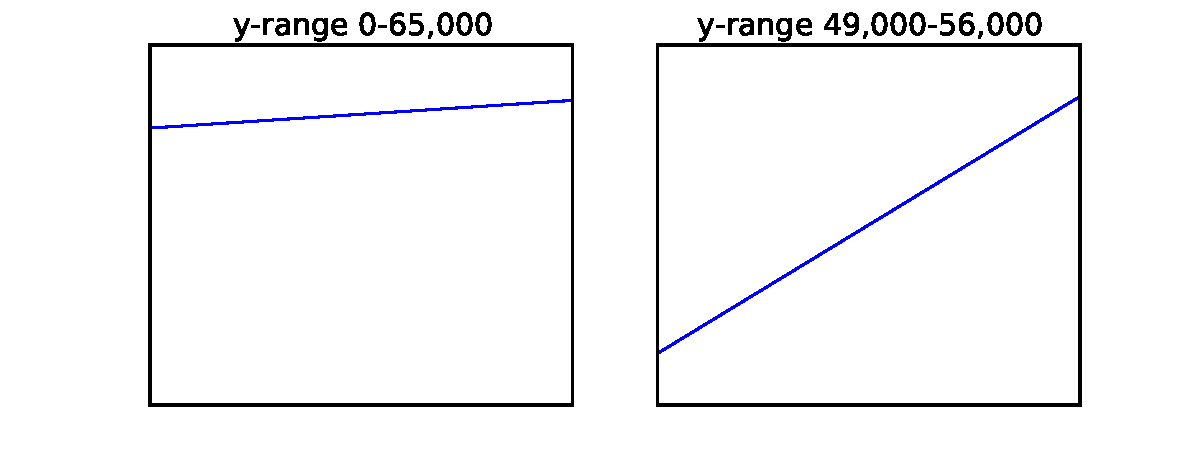
\includegraphics[width=\textwidth]{dog_plots.pdf}
\caption{The graph of some data can look very different depending on the scale. 
Here are two graphs of the ``same'' line over the same range (1 to 4). 
The only difference is the $y$-range. Notice easy it is to manipulate the y-scale to imply either a large or small increase in $y$. 
These figures are especially misleading when we leave the range markers off of the $y$-axes.}
\label{fig:dog_plots}
\end{figure}

Three-dimensional special effects also tend to be misleading. 
A 3-D pie chart, for example, can be used to distort the sizes of its slices. 
Similarly, a 3-D histogram can use perspective to distort the relative differences between bars.

As in any form of communication, integrity is important in data visualization. 
You will win more respect for yourself and those you represent if you avoid misleading diagrams.

\printbibliography